\documentclass{beamer}

\usepackage{amsmath,amssymb,amsfonts}
\usepackage{tikz}
\usetikzlibrary{decorations.pathreplacing}

\usetheme[secheader]{Madrid}

\title[Baby XS]{Baby XS: Just enough to get you started\\YAPC::NA 2012}
\author{Joel Berger}
\institute[UIC]{University of Illinois at Chicago}

\usepackage{pygments}

\providecommand{\subitem}[1]{\begin{itemize}\item#1\end{itemize}}

\begin{document}

\begin{frame}
  \maketitle
\end{frame}

\begin{frame}{Outline}
  \tableofcontents
\end{frame}

\section{Introduction}

\begin{frame}{What is XS?}
  \begin{itemize}
    \item XS links Perl and C
    \item XS is C functions/macros provided by Perl headers
    \item XS is also XS-preprocessesor directives
  \end{itemize}
\end{frame}

\begin{frame}{What are ``baby'' languages?}
  \begin{block}{``Baby'' Langauge}
    The naive code that new programmers write
  \end{block}
  \begin{itemize}
    \item ``Baby Perl''
      \begin{itemize}
        \item no map/grep
        \item no references
        \item avoids \$\_
      \end{itemize}
    \item ``Full XS'' is powerful but is lots to learn
    \item ``Baby XS'' 
     \begin{itemize}
       \item looks like C
       \item behaves like Perl
     \end{itemize}
  \end{itemize}
\end{frame}

\section{Baby XS}

\begin{frame}{Baby XS}
  \begin{block}{}
    Some "easy" idioms and rules-of-thumb to keep XS from becoming overwhelming
  \end{block}
  \begin{itemize}
    \item ignores typemaps
    \item uses Perl datatype functions from perlguts
    \item ignores most of the XSpp commands
    \item ignores stack macros
    \item avoids (most) issues of ``mortalization''
    \item uses a Perl-level function wrapper to munge input/output if needed
  \end{itemize}
\end{frame}

\begin{frame}{Types}
  XS has types that are like their Perl counterparts
  \begin{itemize}
    \item Scalar $\Leftrightarrow$ SV*
    \item Array $\Leftrightarrow$ AV*
    \item Hash $\Leftrightarrow$ HV*
  \end{itemize}
  Of course XS is really C so it also has types like
  \begin{itemize}
    \item int
    \item double
    \item char*
  \end{itemize}
  \ldots which Perl converts to/from SV* when used as arguments or return value
  \begin{block}{For Future Reference}
    You can add you own automatic conversions via a \alert{Typemap} file
  \end{block}
\end{frame}

\section{The Code}

\begin{frame}[fragile]{Full Code (lib/My/Module.xs)}
  \tiny
  \begin{columns}
    \begin{column}{0.49\linewidth}
      \begin{Verbatim}[commandchars=\\\{\}]
\PY{c+cp}{\PYZsh{}}\PY{c+cp}{include "EXTERN.h"}
\PY{c+cp}{\PYZsh{}}\PY{c+cp}{include "perl.h"}
\PY{c+cp}{\PYZsh{}}\PY{c+cp}{include "XSUB.h"}

\PY{k+kt}{int} \PY{n+nf}{meaning} \PY{p}{(}\PY{p}{)} \PY{p}{\PYZob{}} \PY{k}{return} \PY{l+m+mi}{42} \PY{p}{\PYZcb{}}
\PY{k+kt}{void} \PY{n+nf}{greet} \PY{p}{(}\PY{k+kt}{char}\PY{o}{*} \PY{n}{name}\PY{p}{)} 
\PY{p}{\PYZob{}}
  \PY{n}{printf}\PY{p}{(} \PY{l+s}{"}\PY{l+s}{Hello \PYZpc{}s}\PY{l+s+se}{\PYZbs{}n}\PY{l+s}{"}\PY{p}{,} \PY{n}{name} \PY{p}{)} 
\PY{p}{\PYZcb{}}

\PY{n}{MODULE} \PY{o}{=} \PY{n}{My}\PY{o}{:}\PY{o}{:}\PY{n}{Module}    \PY{n}{PACKAGE} \PY{o}{=} \PY{n}{My}\PY{o}{:}\PY{o}{:}\PY{n}{Module}

\PY{k+kt}{int}
\PY{n}{meaning} \PY{p}{(}\PY{p}{)}

\PY{k+kt}{void}
\PY{n}{greet} \PY{p}{(}\PY{n}{name}\PY{p}{)}
    \PY{k+kt}{char}\PY{o}{*} \PY{n}{name}
\end{Verbatim}

    \end{column}
    \begin{column}{0.49\linewidth}
      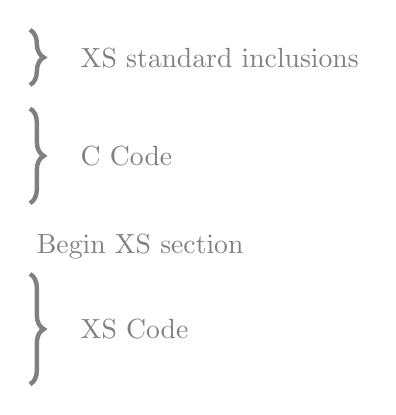
\begin{tikzpicture}
        \visible<2->{
          \draw
            [decoration={brace,amplitude=0.5em},decorate,ultra thick,gray]
            (0,2) --
            (0,1.3)
              node [right=5mm,pos=0.5] {XS standard inclusions}
          ;
        }
        \visible<3->{
          \draw
            [decoration={brace,amplitude=0.5em},decorate,ultra thick,gray]
            (0,1) --
            (0,-0.2)
              node [right=5mm,pos=0.5] {C Code}
          ;
        }
        \visible<4->{
          \node at (1.4,-0.75) [gray] {Begin XS section};
        }
        \visible<5->{
          \draw
            [decoration={brace,amplitude=0.5em},decorate,ultra thick,gray]
            (0,-1.1) --
            (0,-2.5)
              node [right=5mm,pos=0.5] {XS Code}
          ;
        }
      \end{tikzpicture}
    \end{column}
  \end{columns}
\end{frame}

\end{document}
